\documentclass[10pt,fleqn]{article} % Default font size and left-justified equations
\usepackage[%
    pdftitle={Modélisation dynamique},
    pdfauthor={Xavier Pessoles}]{hyperref}

\input{../../../style/packages}
\input{../../../style/new_style}
\input{../../../style/macros_SII}
\input{../../../style/environment}
% Déclaration des titres
% -------------------------------------


\graphicspath{{../../../style/png/}{images/}{../../../Informatique/exercices/consignes/consignes_tp1/}{../../../Informatique/exercices/20_architecture/ARCHI-002/}{../../../Informatique/exercices/01_python_bases/PYB-002-bis/}{../../../Informatique/exercices/01_python_bases/PYB-003-bis/}{../../../Informatique/exercices/01_python_bases/PYB-004/}}
\lstinputpath{{../../../Informatique/exercices/consignes/consignes_tp1/}{../../../Informatique/exercices/20_architecture/ARCHI-002/}{../../../Informatique/exercices/01_python_bases/PYB-002-bis/}{../../../Informatique/exercices/01_python_bases/PYB-003-bis/}{../../../Informatique/exercices/01_python_bases/PYB-004/}}

\def\discipline{Informatique}
\def\xxtete{Informatique}

\def\classe{\textsf{MPSI}}
\def\xxnumpartie{1}
\def\xxpartie{}
\def\xxdate{9 Septembre 2021}

\def\xxchapitre{1}
\def\xxnumchapitre{1}
\def\xxnomchapitre{Prise en main}
\def\xxnumactivite{01}

\def\xxposongletx{2}
\def\xxposonglettext{1.45}
\def\xxposonglety{19}%16

\def\xxonglet{\textsf{Cycle 01}}
\def\xxauteur{\textsl{E. Durif -- X. Pessoles \\ J.P. Berne }}


\def\xxpied{%
Cycle \xxnumpartie -- \xxpartie\\
Chapitre \xxnumchapitre -- \xxactivite -\xxnumactivite -- \xxnomchapitre%
}

\setcounter{secnumdepth}{5}
\chapterimage{Fond_ALG}
\def\xxfigures{}

\def\xxcompetences{%
\textsl{%
%\vspace{-.5cm}
\textbf{Savoirs et compétences :}\\
\vspace{-.1cm}
\begin{itemize}[label=\ding{112},font=\color{ocre}]
\item AA.C01 : Manipuler un OS ou un IDE
\item AA.S01 : Se familiariser aux principaux composants d'une machine numérique
\item AA.S2 : Se familiariser à la manipulation d'un OS
\item AA.S3 : Se familiariser à la manipulation d'un IDE
\end{itemize}
}}


%Infos sur les supports
\def\xxtitreexo{Prise en main}
\def\xxsourceexo{\hspace{.2cm} \footnotesize{\textbf{Sources : }




}}
%\def\xxtitreexo{Titre EXO}
%\def\xxsourceexo{\hspace{.2cm} \footnotesize{Source EXO}}


%---------------------------------------------------------------------------



\usepackage{amsmath}

\livretfalse



\begin{document}
% Sujet
%\TPtrue \fichefalse \proffalse \tdfalse \coursfalse \collefalse
%\corrigefalse
\graphicspath{{../../../style/png/}{images/}{../../../Informatique/S2_Cours/06_BaseGraphes/06_BaseGraphes/images}}


%%%% Paramétrage du cours %%%%
\def\xxactivite{TP}
\def\xxauteur{\textsl{É. Durif -- X. Pessoles -- J.-P. Berne}}
%\fichefalse
%\proftrue
%\tdfalse
%\courstrue

\def\xxYCartouche{-2.25cm}
\def\xxYongletGarde{.5cm}
\def\xxYOnget{.9cm}

\def\xxtitreexo{Découverte de la représentation des graphes}

% Déclaration des titres
% -------------------------------------


\graphicspath{{../../../style/png/}{images/}{../../../Informatique/exercices/consignes/consignes_tp1/}{../../../Informatique/exercices/20_architecture/ARCHI-002/}{../../../Informatique/exercices/01_python_bases/PYB-002-bis/}{../../../Informatique/exercices/01_python_bases/PYB-003-bis/}{../../../Informatique/exercices/01_python_bases/PYB-004/}}
\lstinputpath{{../../../Informatique/exercices/consignes/consignes_tp1/}{../../../Informatique/exercices/20_architecture/ARCHI-002/}{../../../Informatique/exercices/01_python_bases/PYB-002-bis/}{../../../Informatique/exercices/01_python_bases/PYB-003-bis/}{../../../Informatique/exercices/01_python_bases/PYB-004/}}

\def\discipline{Informatique}
\def\xxtete{Informatique}

\def\classe{\textsf{MPSI}}
\def\xxnumpartie{1}
\def\xxpartie{}
\def\xxdate{9 Septembre 2021}

\def\xxchapitre{1}
\def\xxnumchapitre{1}
\def\xxnomchapitre{Prise en main}
\def\xxnumactivite{01}

\def\xxposongletx{2}
\def\xxposonglettext{1.45}
\def\xxposonglety{19}%16

\def\xxonglet{\textsf{Cycle 01}}
\def\xxauteur{\textsl{E. Durif -- X. Pessoles \\ J.P. Berne }}


\def\xxpied{%
Cycle \xxnumpartie -- \xxpartie\\
Chapitre \xxnumchapitre -- \xxactivite -\xxnumactivite -- \xxnomchapitre%
}

\setcounter{secnumdepth}{5}
\chapterimage{Fond_ALG}
\def\xxfigures{}

\def\xxcompetences{%
\textsl{%
%\vspace{-.5cm}
\textbf{Savoirs et compétences :}\\
\vspace{-.1cm}
\begin{itemize}[label=\ding{112},font=\color{ocre}]
\item AA.C01 : Manipuler un OS ou un IDE
\item AA.S01 : Se familiariser aux principaux composants d'une machine numérique
\item AA.S2 : Se familiariser à la manipulation d'un OS
\item AA.S3 : Se familiariser à la manipulation d'un IDE
\end{itemize}
}}


%Infos sur les supports
\def\xxtitreexo{Prise en main}
\def\xxsourceexo{\hspace{.2cm} \footnotesize{\textbf{Sources : }




}}
%\def\xxtitreexo{Titre EXO}
%\def\xxsourceexo{\hspace{.2cm} \footnotesize{Source EXO}}


%---------------------------------------------------------------------------



\input{../../../Style/pagegarde_info_tp.tex}
\setlength{\columnseprule}{.1pt}

\pagestyle{fancy}
\thispagestyle{plain}


\vspace{3.5cm}

\def\columnseprulecolor{\color{ocre}}
\setlength{\columnseprule}{0.4pt} 

%%%%%%%%%%%%%%%%%%%%%%%


\vspace{3cm}

%\begin{multicols}{2}
\graphicspath{{../../../style/png/}{images/}{../../../Informatique/Exercices/S2_06_Graphes/04_Implementation_graphes_matrice/}}
\exer{Implémentation des graphes par une matrice d'adjacence}


On considère le graphe \texttt{G} suivant, où le nombre situé sur l'arête joignant deux sommets est leur distance, supposée entière. 

\begin{center}
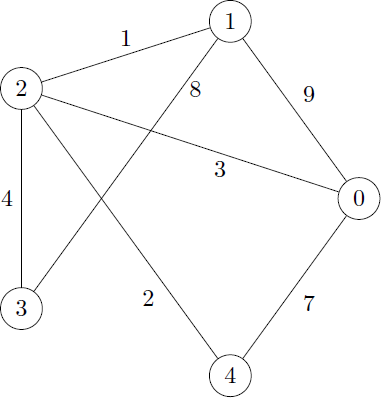
\includegraphics[width=7cm]{images/application_matrice}
\end{center}


\question{Construire la matrice $\left( G_{ij}\right)_{0\leq i,j\leq 4}$, matrice de distances du graphe \texttt{G}, définie par :
<< pour tous les indices $i$, $j$, $G_{ij}$ représente la distance entre les sommets $i$ et $j$,
ou encore la longueur de l'arête reliant les sommets $i$ et~$j$~>>. Cette matrice sera implémentée sous forme d'une liste de listes. (Chaque << sous-liste >> représentant une ligne de la matrice d'adjacence. 
On convient que, lorsque les sommets ne sont pas reliés, cette distance vaut $-1$. La distance du
sommet $i$ à lui-même est égale à 0.}


%\question{Écrire une suite d'instructions permettant de dresser à partir de la matrice \texttt{M} la liste des voisins du sommet 4.}

\question{Écrire une fonction \texttt{voisins(G:list, i:int) -> list}, d'argument la matrice d'adjacence \texttt{G} et un sommet $i$, renvoyant la liste des voisins du sommet~$i$.}


\question{Écrire une fonction \texttt{arretes(G:list) -> list}, renvoyant la liste des arêtes. Les arêtes seront constitués de couples de sommets (l'arête entre les sommets 0 et 1 sera donnée par \texttt{(0,1)}.}

Les instructions suivantes permettent de tracer un graphe. 

\begin{lstlisting}
import networkx as nx

def plot_graphe(G):
    Gx = nx.Graph()
    edges = arretes(G)
    Gx.add_edges_from(edges)
    nx.draw(Gx,with_labels = True)
    plt.show()
plot_graphe(M)
\end{lstlisting}

\question{Écrire et tester la fonction \texttt{plot\_graphe(G)}.}

\question{Écrire une fonction \texttt{degre(G:list, i:int) -> int}, d'argument un sommet $i$, renvoyant le nombre des voisins du sommet $i$, c'est-à-dire le nombre d’arêtes issues de $i$.}


\question{Écrire une fonction \texttt{longueur(G:list,L:list) -> int}, d’argument une liste \texttt{L} de sommets de \texttt{G}, renvoyant la longueur du trajet d'écrit par cette liste \texttt{L}, c’est-à-dire la somme des longueurs des arêtes empruntées. Si le trajet n'est pas possible, la fonction renverra $-1$.}

\question{Écrire la fonction \texttt{ajout\_sommet(G:list, L:list, poids : list) -> None} permettant d'ajouter un sommet au graphe. \texttt{L} désigne la liste des sommets auxquels le nouveau sommet est relié, \texttt{poids} la liste des poids respectifs. \texttt{ajout\_sommet} agit avec effet de bord sur \texttt{G}.}

\question{Écrire la fonction \texttt{supprime\_sommet(G:list, i: int) -> None} permettant de supprimer le sommet $i$ du graphe.}
%
%
%\subsubsection*{Implémentation d'un graphe par une liste d'adjacence}
%Pour implémenter le graphe, on utilise une liste \texttt{G} qui a pour taille le nombre de sommets. Chaque élément \texttt{G[i]} est la liste des voisins de \texttt{i}. 
%
%On s'intéresse au graphe précédent, \textbf{sans les pondérations}.  Dans ce cas, \texttt{G[0]=[1,2,4]} car Les sommets 1, 2 et 4 sont des voisins de 0.
%
%\question{Construire la liste d'adjacence \texttt{G} en utilisant la méthode énoncée ci-dessus.}
%
%\question{Écrire une fonction \texttt{voisins\_l(G:list, i:int) -> list}, d'argument la liste d'adjacence \texttt{G} et un sommet $i$, renvoyant la liste des voisins du sommet~$i$.}
%
%\question{Écrire une fonction \texttt{degre\_l(G:list, i:int) -> int}, d'argument un sommet $i$, renvoyant le nombre des voisins du sommet $i$, c'est-à-dire le nombre d’arêtes issues de $i$.}
%
%\question{Écrire la fonction \texttt{ajout\_sommet\_l(G:list, L:list) -> None} permettant d'ajouter un sommet au graphe. Cette fonction prendra comme argument \texttt{G} liste d'adjacence du graphe et \texttt{L} la liste des sommets auxquels le nouveau sommet est relié. \texttt{ajout\_sommet} agit avec effet de bord sur \texttt{G}.}
%
%\question{Écrire la fonction \texttt{supprime\_sommet\_l(G:list, i: int) -> None} permettant de supprimer le sommet $i$ du graphe.}

\graphicspath{{../../../style/png/}{images/}{../../../Informatique/Exercices/S2_06_Graphes/05_Implementation_graphes_liste/}}
\exer{Implémentation des graphes par une liste d'adjacence}


On considère le graphe \texttt{G} suivant, où le nombre situé sur l'arête joignant deux sommets est leur distance, supposée entière. 

\begin{center}
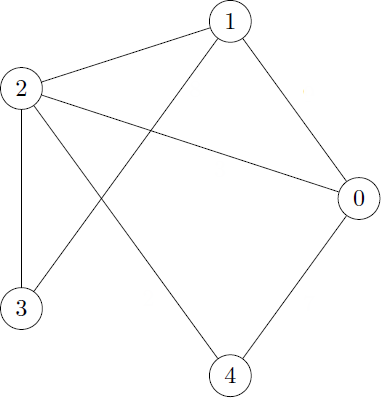
\includegraphics[width=7cm]{images/application_liste}
\end{center}


Pour implémenter le graphe, on utilise une liste \texttt{G} qui a pour taille le nombre de sommets. Chaque élément \texttt{G[i]} est la liste des voisins de \texttt{i}. 

Dans ce cas, \texttt{G[0]=[1,2,4]} car Les sommets 1, 2 et 4 sont des voisins de 0.

\question{Construire la liste d'adjacence \texttt{G} en utilisant la méthode énoncée ci-dessus.}

%
%On convient que, lorsque les sommets ne sont pas reliés, cette distance vaut $-1$. La distance du
%sommet $i$ à lui-même est égale à 0.

%\question{Écrire une suite d'instructions permettant de dresser à partir de la matrice \texttt{M} la liste des voisins du sommet 4.}

\question{Écrire une fonction \texttt{voisins\_l(G:list, i:int) -> list}, d'argument la liste d'adjacence \texttt{G} et un sommet $i$, renvoyant la liste des voisins du sommet~$i$.}


\question{Écrire une fonction \texttt{arretes\_l(G:list) -> list}, renvoyant la liste des arêtes. Les arêtes seront constitués de couples de sommets (l'arête entre les sommets 0 et 1 sera donnée par \texttt{(0,1)}.}

Les instructions suivantes permettent de tracer un graphe. 

\begin{lstlisting}
import networkx as nx

def plot_graphe_l(G):
    Gx = nx.Graph()
    edges = arretes_l(G)
    Gx.add_edges_from(edges)
    nx.draw(Gx,with_labels = True)
    plt.show()
plot_graphe(M)
\end{lstlisting}

\question{Écrire et tester la fonction \texttt{plot\_graphe\_l(G)}.}

\question{Écrire une fonction \texttt{degre\_l(G:list, i:int) -> int}, d'argument un sommet $i$, renvoyant le nombre des voisins du sommet $i$, c'est-à-dire le nombre d’arêtes issues de $i$.}

%\question{Écrire une fonction \texttt{longueur\_l(G:list,L:list) -> int}, d’argument une liste \texttt{L} de sommets de \texttt{G}, renvoyant la longueur du trajet d'écrit par cette liste \texttt{L}, c’est-à-dire la somme des longueurs des arêtes empruntées. Si le trajet n'est pas possible, la fonction renverra $-1$.}

\question{Écrire la fonction \texttt{ajout\_sommet\_l(G:list, L:list) -> None} permettant d'ajouter un sommet au graphe. \texttt{L} désigne la liste des sommets auxquels le nouveau sommet est relié. \texttt{ajout\_sommet} agit avec effet de bord sur \texttt{G}.}

\question{Écrire la fonction \texttt{supprime\_sommet\_l(G:list, i: int) -> None} permettant de supprimer le sommet $i$ du graphe.}


\question{Écrire la fonction \texttt{from\_list\_to\_matrix(G:list, i: int) -> list} permettant de convertir un graphe implémenté sous forme de liste d'adjacence en matrice d'adjacence.}

\question{Écrire la fonction \texttt{from\_matrix\_to\_listmatrix(G:list, i: int) -> list} permettant de convertir un graphe implémenté sous forme de matrice d'adjacence en liste d'adjacence.}


\subsection*{Exercices d'application sur les piles}

Dans les exercices qui suivent, on utilisera des \textbf{piles}. Les piles sont des structures de données basées sur le principe LIFO (Last In First Out : le dernier rentré dans la pile sera le premier à en sortir).

Les opérations élémentaires qu'on peut réaliser sur les piles sont les suivantes : 
\begin{itemize}
\item savoir si une pile est vide; 
\item empiler un nouvel élément sur la pile;
\item récupérer l'élément au sommet de la pile tout en le supprimant. On dit que l'on dépile;
\item accéder à l'élément situé au sommet de la pile sans le supprimer de la pile;
\item on peut connaitre le nombre d'éléments présents dans la pile.
\end{itemize}

Pour implémenter les piles on utilisera le module \texttt{deque}. Chacun des éléments de la pile peut être un objet de type différent.

\begin{lstlisting} 
from collections import deque

# Créer une pile vide
pile = deque() 

# Tester si une pile est vide
len(pile) == 0

# Ajouer l'élément Truc au sommet de la pile
pile.append("Truc")

# Supprimer (et renvoyer) le sommet d'une pile non vide
sommet = pile.pop()
\end{lstlisting}


\textbf{Seules ces fonctions éléméntaires seront utilisées dans les exercices suivants.}

\exer{La parenthèse inattendue}
Dans cet exercice, on souhaite savoir si une chaîne de caractères est bien parenthésée ou non. 
Une chaîne bien parenthésée est une chaîne vide ou la concaténation de chaînes bien parenthésées. 
\begin{exemple}
Chaînes bien parenthésées :
\begin{itemize}
\item \texttt{"()"},\texttt{"()()"},\texttt{"(())"} et \texttt{"(()())"}.
\end{itemize}
Chaînes mal parenthésées :
\begin{itemize}
\item \texttt{")("},\texttt{"(("},\texttt{"(()"} et \texttt{"())"}.
\end{itemize}
\end{exemple} 

\question{Implémenter la fonction \texttt{parentheses} répondant aux spécifications suivantes : }

\begin{lstlisting} 
def parenthese(s):
    "
    Retourne les couples d'indice parenthèse 
    ouvrante, parenthèse fermante.
    Entrée :
     * s(str) : chaîne de caractères bien 
     parenthésée constituée uniquement 
     de parenthèses.
    Sortie : 
     * Affichage des couples d'indices.
    "
\end{lstlisting}
\ifprof
\begin{corrige}
~\\
\begin{lstlisting} 
def parentheses(s):
    p = creer_pile(len(s))
    for i in range(len(s)):
    if s[i] == '(':
        empiler(p, i)
    else:
        if est_vide(p):
            return False
        j = depiler(p)
        print((j, i))
    return est_vide(p)
\end{lstlisting}
\end{corrige}
\else
\fi

\question{Réaliser un programme permettant de savoir si une chaîne de caractères est bien parenthésée. La structure de pile est-elle nécessaire ?}
\ifprof
\begin{corrige}
\end{corrige}
\else
\fi

\question{Adapter le premier programme pour qu'il puisse traiter des chaînes constituées de parenthèses, de crochets, ou d'accolades. Un mot est alors bien parenthésé si la parenthèse fermante qui correspond à chaque parenthèse ouvrante est du même type.}
\ifprof
\begin{corrige}
\end{corrige}
\else
\fi

\question{Adapter le programme pour qu’il puisse traiter des mots constitués de parenthèses et
d’autres caractères, qui n’interfèrent pas avec les parenthèses.}
\ifprof
\begin{corrige}
\end{corrige}
\else
\fi

\question{Écrire une version récursive de la fonction \texttt{parentheses}.}
\ifprof
\begin{corrige}
\end{corrige}
\else
\fi

%%%%%%%%%%%%%%

\exer{Inversion}
\subparagraph*{}
\setcounter{exo}{0}

\question{Écrire une fonction qui intervertit les deux éléments situés au sommet d’une pile de taille
au moins égale à 2.}
\ifprof
\begin{corrige}
\end{corrige}
\else
\fi


%%%%%%%%%%%%%%

\exer{Dépile le n\ieme}
\setcounter{exo}{0}

\question{Écrire une fonction qui dépile et renvoie le troisième élément d’une pile de taille au moins
égale à 3. Les premier et deuxième éléments devront rester au sommet de la pile.}
\ifprof
\begin{corrige}
\end{corrige}
\else
\fi

%%%%%%%%%%%%%%

\exer{Lire  le n\ieme}
\setcounter{exo}{0}

\question{Écrire une fonction qui permet de lire (sans l’extraire) le n-ième élément d’une pile. On
prévoira le cas où la pile n’est pas de taille suffisante pour qu’un tel élément existe.}
\ifprof
\begin{corrige}
\end{corrige}
\else
\fi

%\section*{Exercice}
%\setcounter{exo}{0}
%\subparagraph*{}
%\textit{Programmer les fonctions sommet et taille uniquement à l’aide de empiler, depiler et
%est_vide, indépendamment de la réalisation de pile choisie.
%Que peut-on dire de la complexité en temps et en espace de cette fonction taille ?}
%\ifprof
%\begin{corrige}
%\end{corrige}
%\else
%\fi

%%%%%%%%%%%%%%

\exer{Inversion des extrêmes}

\setcounter{exo}{0}
\question{Écrire une fonction qui prend une pile non vide en argument et place l’élément situé à
son sommet tout au fond de la pile, en conservant l’ordre des autres éléments.
Quelle est sa complexité en temps et en espace ?}
\ifprof
\begin{corrige}
\end{corrige}
\else
\fi

%%%%%%%%%%%%%%

\exer{Inversion de la pile}
\setcounter{exo}{0}

\question{Écrire une fonction similaire à \texttt{reversed}, qui prend une pile en argument et renvoie une autre pile constituée des mêmes éléments placés dans l’ordre inverse.}

\question{Si l’on s’autorise à détruire la pile fournie, quelle est la complexité en temps et en espace de cette fonction ? Et si on ne s’y autorise pas ?}
\ifprof
\begin{corrige}
\end{corrige}
\else
\fi

%%%%%%%%%%%%%%

\exer{Tu coupes ?}
\setcounter{exo}{0}

\question{Écrire une fonction couper qui prend une pile et la coupe en enlevant de son sommet un
certain nombre d’éléments (tirés au hasard) qui sont renvoyés dans une seconde pile.}

\begin{exemple}
Si la pile initiale est \texttt{[1, 2, 3, 4, 5]}, et que le nombre d’éléments retiré vaut 2, alors la pile ne contient plus que \texttt{[1, 2, 3]} et la pile renvoyée contient \texttt{[5,4]}.
\end{exemple}
\ifprof
\begin{corrige}
\end{corrige}
\else
\fi

%\end{multicols}

\end{document}